\documentclass[compress]{beamer}
\usepackage[T1]{fontenc}
%\usepackage{newtxtext,newtxmath}
\usepackage{lmodern}% http://ctan.org/pkg/lm
\usepackage{pgfpages}
\usepackage{graphicx}
\usepackage{mathtools}          % used for equations


\mode<presentation>{\usetheme{Darmstadt}}
\usefonttheme{professionalfonts} % using non standard fonts for beamer
\usecolortheme{beaver}
\usecolortheme{rose}
\useoutertheme[footline=empty,subsection=false]{miniframes}
\useinnertheme{default}
\setbeamertemplate{items}[default]
\setbeamertemplate{section in toc}[sections numbered]
\setbeamertemplate{subsection in toc}[sections default]
\beamertemplatenavigationsymbolsempty

\setlength{\unitlength}{\textwidth}  % measure in textwidths


\title[Trajectory optimization]{Energy savings for UAV flight in unsteady gusting conditions \\
through trajectory optimization }
\author{Lou Grimaud} % (optional, for multiple authors)
\institute{Illinois Institute of Technology} % (optional)
\date{July 2014} % (optional)

\logo{
\includegraphics[height=0.3cm]{./Figures/IIT_Logo2.eps}}

\begin{document}
\AtBeginSection[]
{
  \begin{frame}
    \frametitle{Table of Contents}
    \tableofcontents[currentsection,currentsubsection]
  \end{frame}
}


\frame{\titlepage}

\begin{frame}
  \frametitle{Table of Contents}
  \tableofcontents
\end{frame}

\section{Introduction}
\begin{frame}
  \frametitle{Introduction and motivations}

\end{frame}

\section[Trajectory optimization]{The trajectory optimization problem}

\subsection{Dynamic soaring}

\begin{frame}
    \frametitle{Different types of soaring}
  \begin{columns}
    \column{.5\textwidth}
    \begin{figure}[h]
      \centering
      %\includegraphics{<+file+>}
      \caption{something about soaring}
    \end{figure}
    \column{.5\textwidth}
    {\Large Spatial wind gradients}
    \begin{itemize}
      \item Thermal updrafts
      \item Horizontal wind gradients
    \end{itemize}
    {\Large Temporal wind gradients}
    \begin{itemize}
      \item Natural turbulences
      \item Building and natural feature wake
    \end{itemize}
  \end{columns}
\end{frame}

\subsection{Neutral energy loop}

\begin{frame}
  \frametitle{Defining the energy extraction problem}
  \begin{columns}
    \column{.5\textwidth}
    What is an ``optimal trajectory''?
    \begin{itemize}
      \item Maximum energy at the end of the cycle
      \item Maximizing the energy gain at each instant of the cycle
      \item \emph{Minimize the energy input needed for sustainable flight}
    \end{itemize}

    \column{.5\textwidth}
    \begin{block}{The neutral energy loop}
     Finding the minimal wind gust that allows to maintain altitude and speed over a gust. 
    \end{block}
  \end{columns}
\end{frame}

\begin{frame}%[shrink]
  \frametitle{Aircraft model\footnote{\tiny Lissaman P. 43rd AIAA Aerospace Sciences Meeting and Exhibit, 241, 2005.}}
  \begin{equation*}
    \begin{array}[c]{c}
      m \ddot{x} = -L' \cdot sin(\gamma) + D' \cdot cos(\gamma) \\
      m \ddot{z} = L' \cdot cos(\gamma) - D' \cdot sin(\gamma) - m \cdot g
    \end{array}
  \end{equation*}
  \begin{columns}
    \column{.4\textwidth}
    \begin{figure}[h]
      \centering
      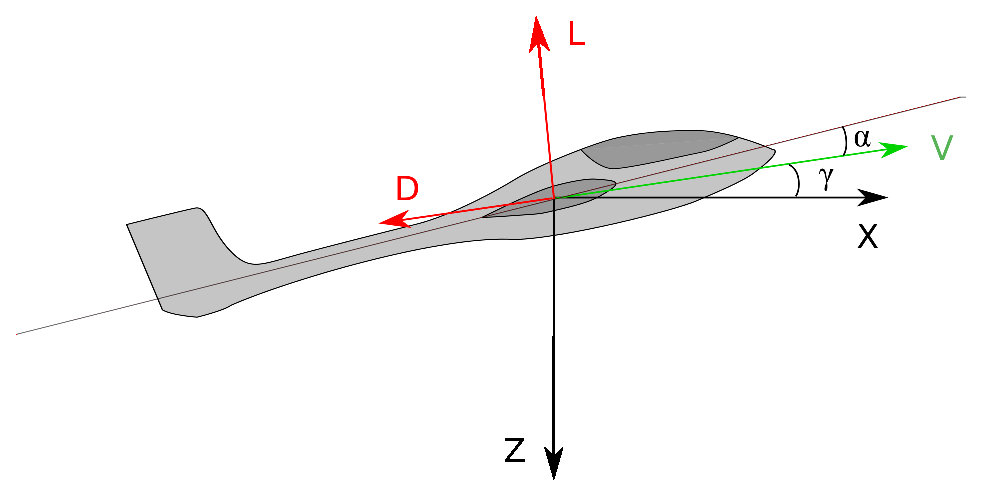
\includegraphics[width=1\textwidth]{./Figures/glider.eps}
      %\caption{Coordinate system used for the optimization}
    \end{figure}
    \column{.7\textwidth}
    Lissaman's non-dimensional variables
    \begin{itemize}
      \item Velocities with $V^{*}$ the optimal glide speed
      \item Time with $T=\frac{V^{*}}{g}$
      \item Lift and drag coefficients $L= \frac{C_l}{C_l^*}$ and $D= \frac{C_d}{C_d^*}$
      \item Dynamic pressure $Q = \frac{L'}{MgL} = \frac{\frac{1}{2} \rho V^2 C_l C_l^* }{Mg}$
    \end{itemize}
  \end{columns}
  \begin{equation*}
    \begin{array}[c]{c}
      \\
      \frac{dU}{dT}= -LQ \cdot sin(\gamma) + DQ \cdot cos(\gamma) \\
      \frac{dW}{dT}= LQ \cdot cos(\gamma) - DQ \cdot sin(\gamma) - 1
    \end{array}
  \end{equation*}
\end{frame}

\begin{frame}
  \frametitle{Quasi-steady lift and drag model}
  \begin{columns}[t]
    \column{.5\textwidth}
    \begin{itemize}
      \item NACA0009 characteristic
    \end{itemize}
    \column{.5\textwidth}
    \begin{itemize}
      \item Lissaman's quadratic drag
    \end{itemize}
  \end{columns}
  \begin{columns}
    \column{.6\textwidth}
	\begin{figure}[h]
	  \centering
	  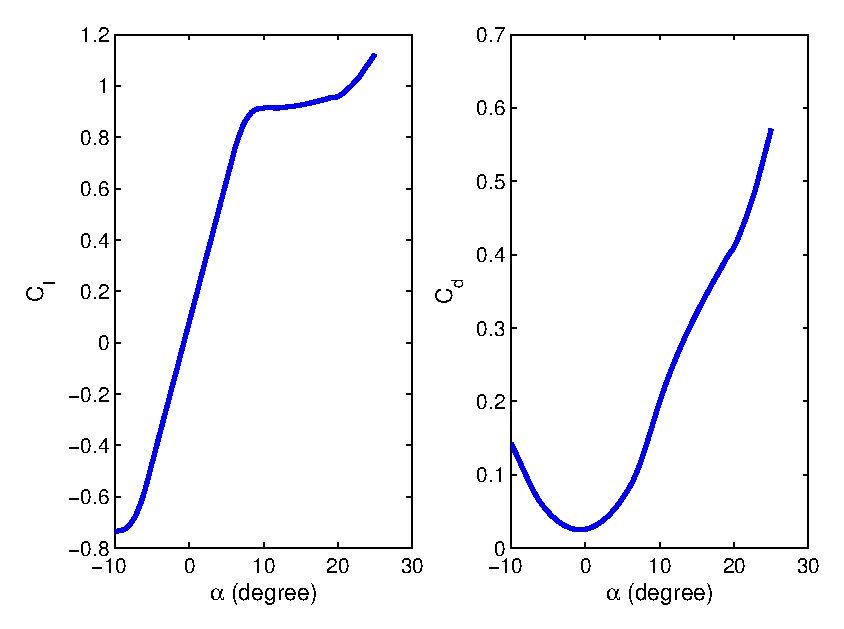
\includegraphics[width=1\textwidth]{./Figures/NACA0009_steady_map_Cl_Cd.eps}
	  \caption{Simplified lift and drag for the NACA0009 airfoil}
	\end{figure}
    \column{.4\textwidth}
	\begin{equation*}
    \begin{array}[c]{c}
	  D=\frac{1+L^2}{2G^*}\\ \\ \\ \\ 
	\end{array}
	\end{equation*}
  \end{columns}
\end{frame}

\begin{frame}
  \frametitle{Wind profiles}
  We define three different wind profiles:
  \begin{itemize}
    \item Vertical wind gust:
      \begin{equation*}
	\begin{array}[c]{c}
	  W_g = W_a \cdot \sin(2\pi T) \\
	  U_g = 0 
	\end{array}
      \end{equation*}
    \item Horizontal wind gust:
      \begin{equation*}
	\begin{array}[c]{c}
	  W_g =0 \\ 
	  U_g = W_a \cdot \cos(2\pi T) 
	\end{array}
      \end{equation*}
    \item Combined wind gust:
      \begin{equation*}
	\begin{array}[c]{c}
	  W_g = W_a \cdot \sin(2\pi T) \\ 
	  U_g = W_a \cdot \cos(2 \pi T + \varphi)
	\end{array}
      \end{equation*}
  \end{itemize}
\end{frame}

\begin{frame}
  \frametitle{Optimization algorithm}
  The cycle is discretized 
  \begin{equation*}
    x= 
    \begin{bmatrix}
      \cdots \\
      X_i \\
      Z_i \\
      U_i \\
      W_i \\
      L_i / \alpha_i \\
      \cdots \\
      W_a
    \end{bmatrix}
    \quad i \in [1,N]
  \end{equation*}

  %state vector and cost function
\end{frame}

\begin{frame}
  \frametitle{Constraints formulation}

\end{frame}

\subsection{Implementation and validation}

\begin{frame}
  \frametitle{Comparison with Lissaman's results}
  \begin{columns}
    \column{0.5\textwidth}
    \begin{figure}[ht]
      \begin{center}	
	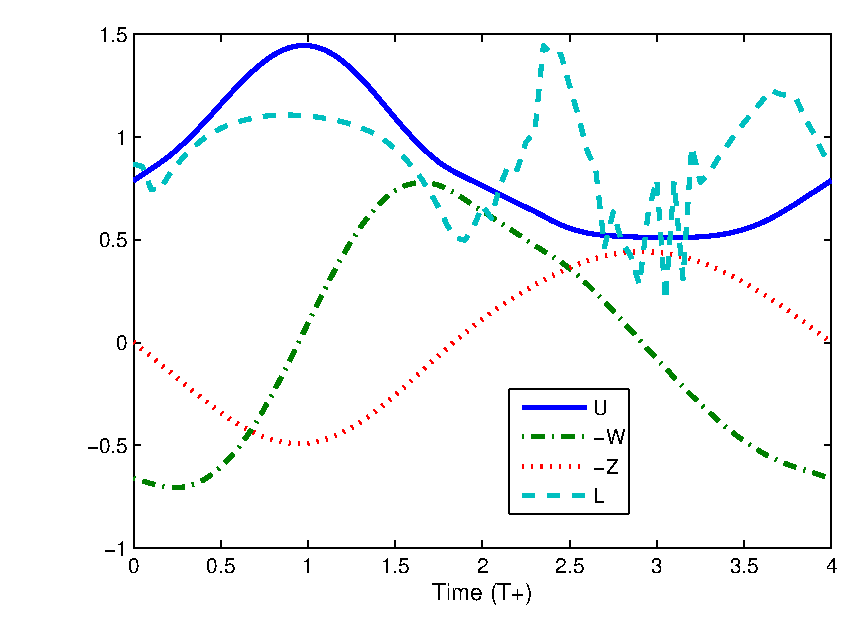
\includegraphics[width=1\textwidth]{./Figures/Windtype=1_Tg=4_Wg=0p129_quad_G=20.eps}
      \end{center}
      \caption{Optimization results for a $4T$ long vertical gust}
      \label{fig:Validation_optimization}
    \end{figure}
    \column{0.5\textwidth}
    \begin{figure}[h]
      \centering
      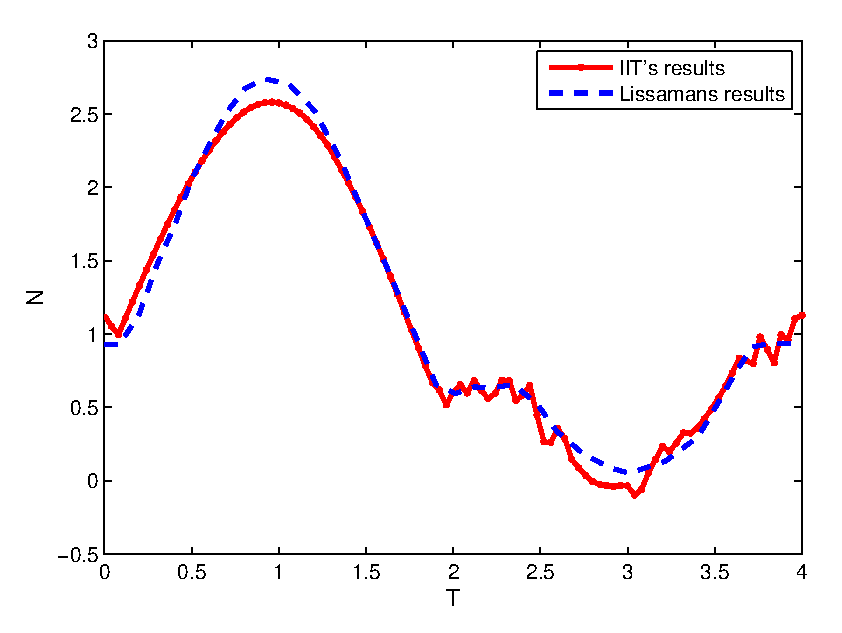
\includegraphics[width=1\textwidth]{./Figures/LIssaman_N_comparison.eps}
      \caption{Comparison with Lissaman's non-dimensional normal force $N$ for a $4T$ long vertical gust}
    \end{figure}
  \end{columns}
  %put the lissaman quadratic thing here
\end{frame}

\begin{frame}
  \frametitle{Quasi-steady lift to drag model}
  \begin{columns}
    \column{0.5\textwidth}
    \begin{figure}
      \begin{center}
	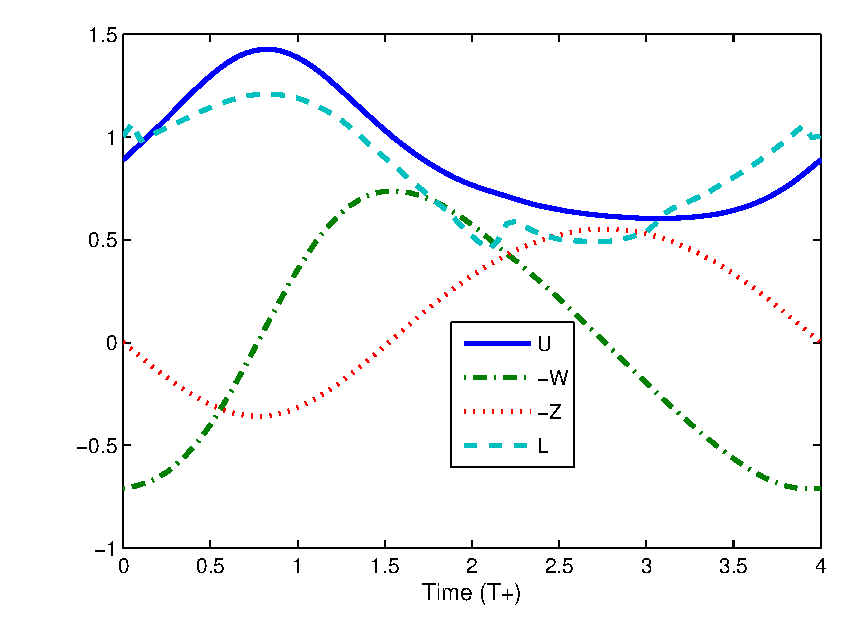
\includegraphics[width=1\textwidth]{./Figures/Windtype=1_Tg=4_Wg=0p205_UAV_alphamax=12.eps}
      \end{center}
      \caption{$4T$ long vertical gust for the NACA0009 airfoil, $W_a=0.205$}
    \end{figure}
    \column{0.5\textwidth}
    \begin{figure}[h]
      \begin{center}
	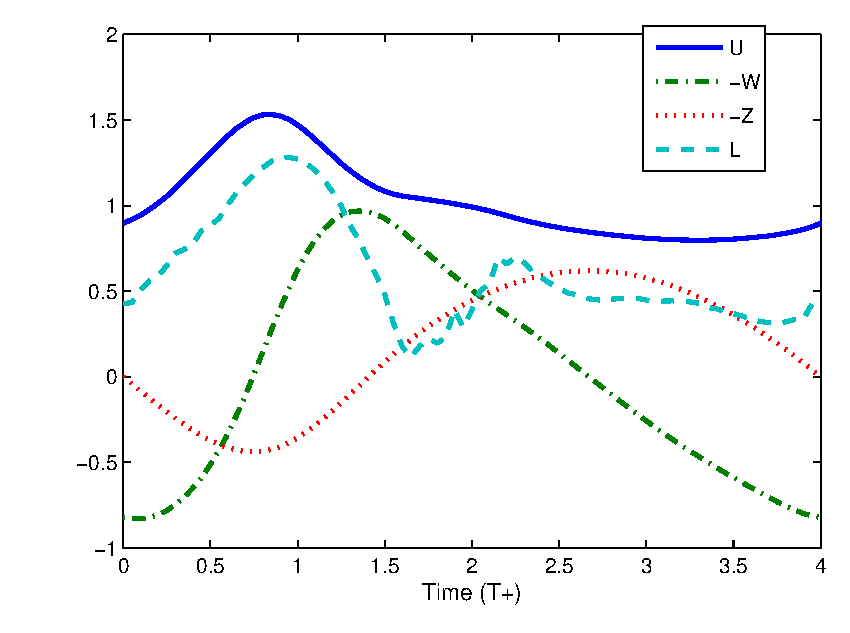
\includegraphics[width=1\textwidth]{./Figures/Windtype=3_Tg=4_Wg=0p387_UAV_alphamax=12.eps}
      \end{center}
      \caption{$4T$ long combined gust for the NACA0009 airfoil, $W_a=0.387$}
    \end{figure}
  \end{columns} % NACA009 curves
\end{frame}

\subsection{Quasi-steady aerodynamic model results}

\begin{frame}
  \frametitle{Tg dependency}
  \begin{columns}
    \column{0.5\textwidth}
    \begin{figure}[h!]
      \begin{center}
	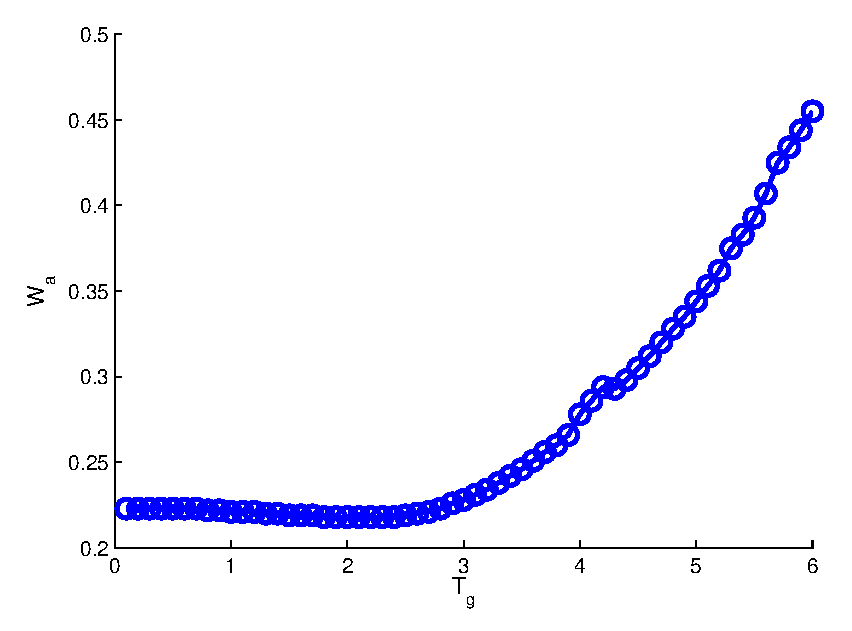
\includegraphics[width=1\textwidth]{./Figures/Wg_vs_TG_windtype=1_alhpamax=12_nodalphalimit.eps}
      \end{center}
      \caption{Influence of gust duration on the minimum gust amplitude for vertical gusts}
      \label{fig:vertical_amplitude_duration}
    \end{figure}
    \column{0.5\textwidth}
    \begin{figure}[h!]
      \begin{center}
	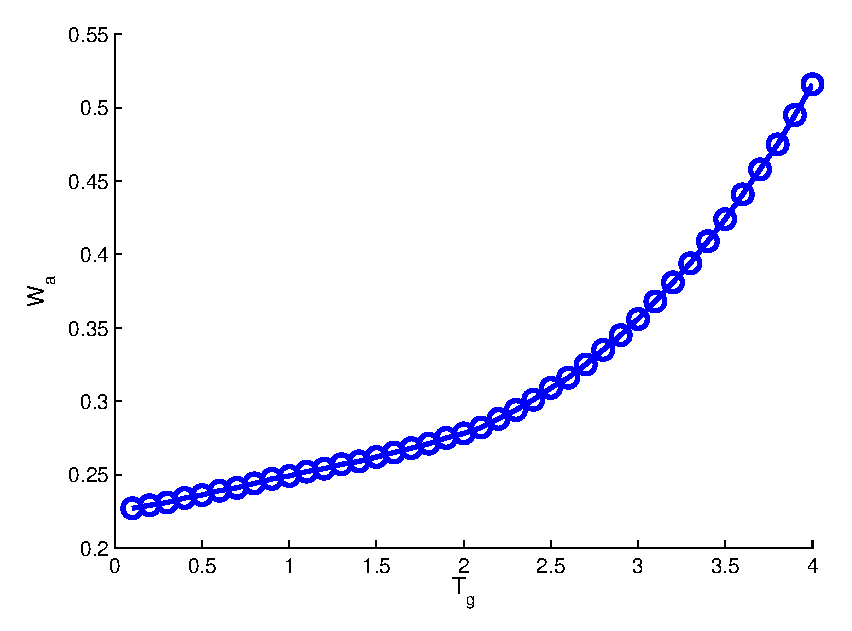
\includegraphics[width=1\textwidth]{./Figures/Wg_vs_TG_windtype=3_alhpamax=12_nodalphalimit.eps}
      \end{center}
      \caption{Influence of gust duration on the minimum gust amplitude for combined gusts}
      \label{fig:combined_amplitude_duration}
    \end{figure}
  \end{columns} % NACA009 curves
\end{frame}

\begin{frame}
  \frametitle{Difference between short and long gusts}
We can see that there is tipping point around $T_g=2.5$
\begin{figure}[h]
  \centering
  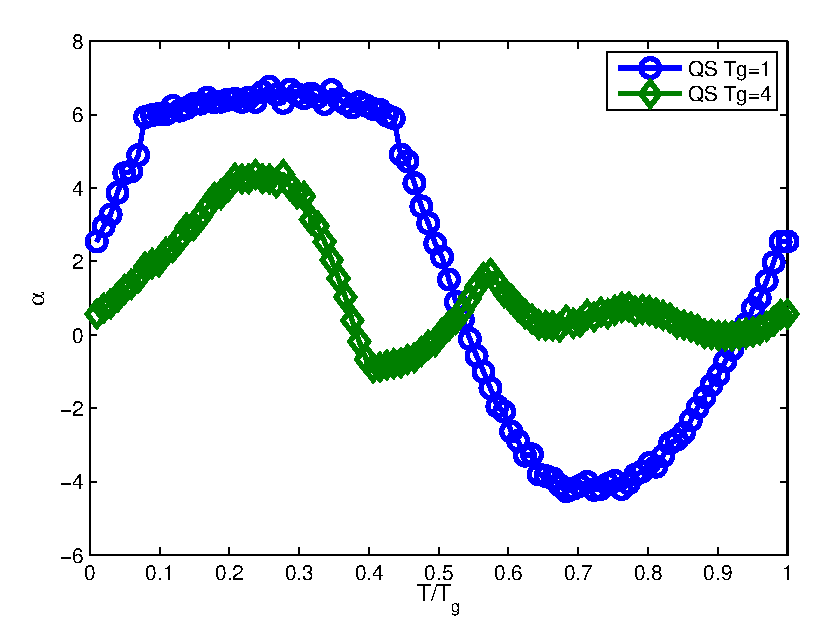
\includegraphics[width=0.7\textwidth]{./Figures/alpha_vs_Tg_QS_short_vs_long_wt3.eps}
  \caption{Difference between short and long gust angle of attack profile for combined gusts}
  \label{fig:short_vs_long_qs_wt=3}
\end{figure}
\end{frame}

\begin{frame}
  \frametitle{Angle of attack limitation}
  \begin{columns}
    \column{0.5\textwidth}
    \begin{figure}[h]
      \centering
      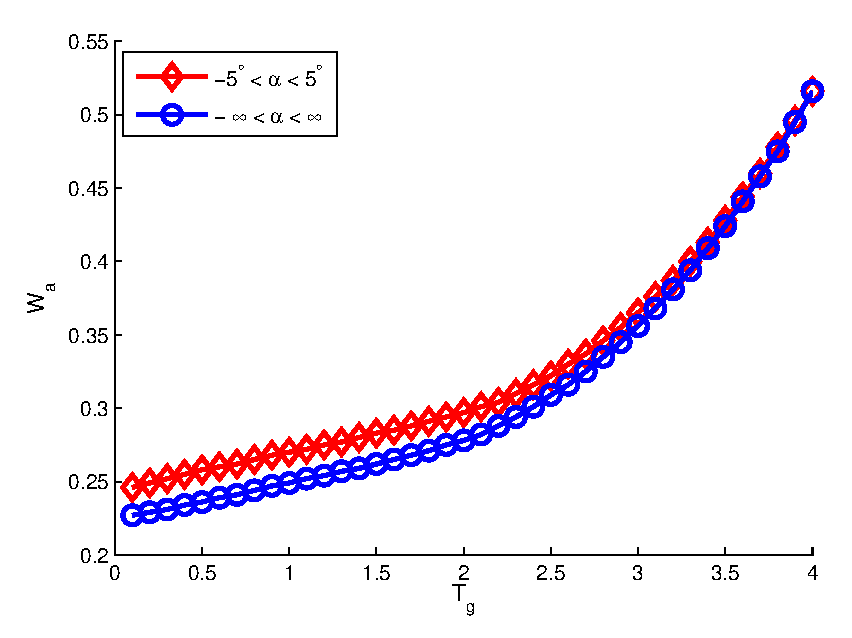
\includegraphics[width=1\textwidth]{./Figures/allowed_alpha_wg_tg_wt=3.eps}
      \caption{Difference in performance for combined wind gusts if no high angle of attack are allowed}
      \label{fig:allowed_alpha_Wt_vs_tg_wt=3}
    \end{figure}

    \column{0.5\textwidth}
    \begin{figure}[h]
      \centering
      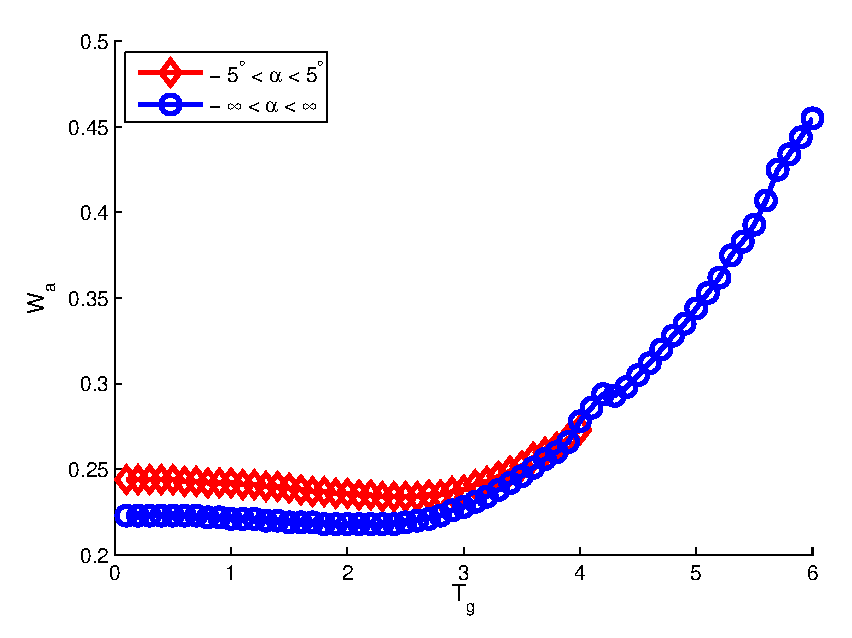
\includegraphics[width=1\textwidth]{./Figures/allowed_alpha_wg_tg_wt=1.eps}
      \caption{Difference in performance for vertical wind gusts if no high angle of attack are allowed}
      \label{fig:allowed_alpha_Wt_vs_tg_wt=1}
    \end{figure}
  \end{columns}
\end{frame}

\begin{frame}
  \frametitle{Phase influence}
\begin{figure}[ht]
  \begin{center}
    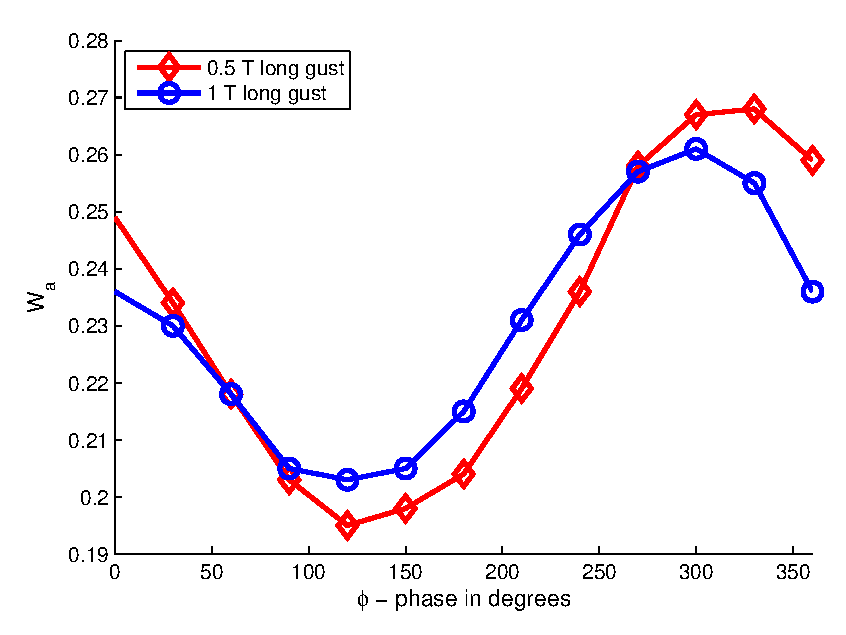
\includegraphics[width=0.7\textwidth]{./Figures/combined_gust_amplitude_vs_phase_LUT.eps}
  \end{center}
  \caption{Influence of the phase between the components of the combined gust}
  \label{fig:combined_amplitude_phase}
\end{figure}
\end{frame}


\section[GK model]{The unsteady pitching aerodynamic model}

\subsection{Experimental setup}

\begin{frame}[shrink]
  \frametitle{Pitching mechanism and experimental conditions}
  \begin{columns}
    \column{0.6\textwidth}
    \begin{figure}[h]
      \begin{center}
	\includegraphics[width=1.0\textwidth]{./Figures/airfoil_model.eps}
      \end{center}
      \caption{Airfoil model inside the wind tunnel}
    \end{figure}
    \column{0.5\textwidth}
    Experimental conditions
    \begin{itemize}
      \item Free stream velocity: 3 m/s
      \item Airfoil: NACA0009
      \item Reynolds number ~50000
    \end{itemize}
    Controller and data acquisition
    \begin{itemize}
      \item Angle of attack controlled by simulink\textsuperscript{\textregistered} and two servomotors 
      \item Servos position measured by two linear potentiometers
      \item Piezoelectric force balance (NANO17) to measure the forces on the airfoil
    \end{itemize}
  \end{columns}
\end{frame}

\subsection{The Goman and Khrabrov model}

\begin{frame}
  \frametitle{The GK model concept}
  The Goman and Khrabrov model\footnote{Goman M and Khrabrov A. \emph{Journal of Aircraft}, 31(5):1109–1115,1994.} - a non-linear state space model
  \begin{equation*}
    \begin{array}[c]{c}
      C_l= f(\alpha,x(\alpha)) \\
      C_d= g(\alpha,x(\alpha)) \\
      \tau_1 \frac{dx}{dt} +x = x_0(\alpha - \tau_2 \dot{\alpha}) 
    \end{array}
  \end{equation*}

  \begin{columns}[t] 
    \column{0.38\textwidth}
      \begin{itemize}
      \item   \textbf{Lift and drag model}
    \end{itemize}
    \column{0.38\textwidth}
     \begin{itemize}
      \item    \textbf{Non-linear state map}
    \end{itemize}
    \column{0.38\textwidth}
    \begin{itemize}
      \item \textbf{Time constants $\tau_1$ and $\tau_2$} 
    \end{itemize}
  \end{columns}

  \begin{columns}
    \column{0.4\textwidth}
    \resizebox{\textwidth}{!}{%
      $
      \begin{array}[c]{c}
	\\
	C_l=2 \pi \alpha (0.6 x + 0.4) + C_{l0} \\
	C_d= \frac{ \left( \left( 2 - x \right)C_l \right)^2 }{G_{\max}} + C_{d0}
      \end{array}
      $%
    }
    \column{0.4\textwidth}
    \begin{figure}[h]
      \begin{center}
	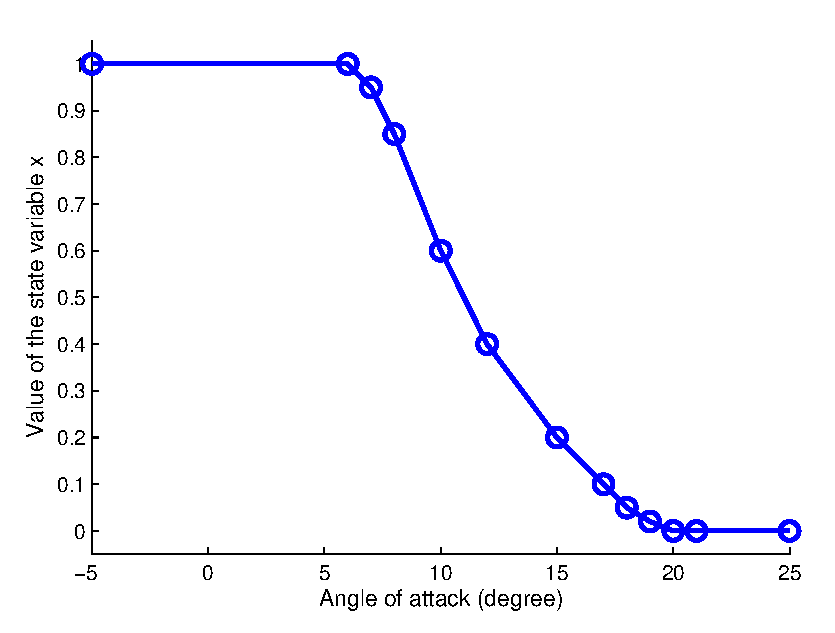
\includegraphics[width=0.9\textwidth]{./Figures/x_0_vs_alpha.eps}
      \end{center}
    \end{figure}
    \column{0.4\textwidth}
    \begin{figure}[h]
      \begin{center}
	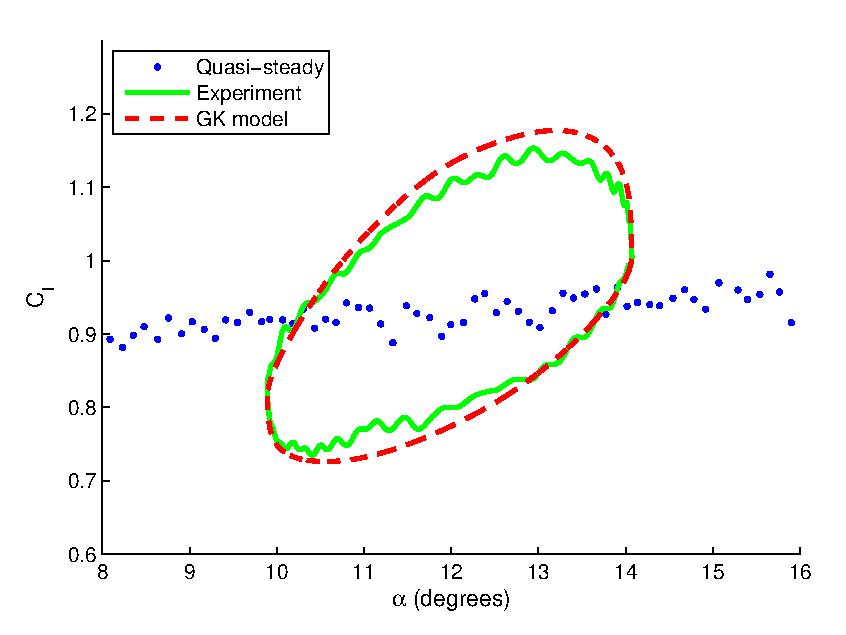
\includegraphics[width=0.9\textwidth]{./Figures/Cl_u=3_meanaoa=12_amp=2_freq=0p5.eps}
      \end{center}
    \end{figure}

  \end{columns}
\end{frame}

\subsection{Determination and validation of the model}

\begin{frame}
  \frametitle{Quasi-steady map and state variable}
\begin{equation*}
  C_l(\alpha,x)=2 \pi \cdot \alpha (0.6 x + 0.4) + C_{l0}
\end{equation*}
  \begin{columns}
    \column{0.5\textwidth}
    \begin{figure}[h]
      \begin{center}
	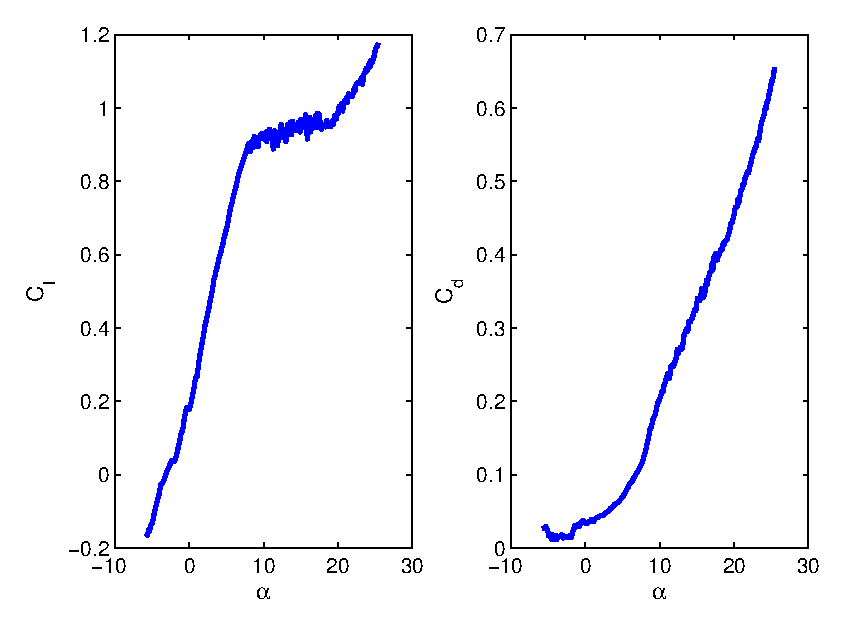
\includegraphics[width=1\textwidth]{./Figures/Cd_and_Cl_NACA0009.eps}
      \end{center}
      \caption{Lift and drag coefficient in the quasi-steady case}
    \end{figure}
    \column{0.5\textwidth}
    \begin{figure}[ht]
      \begin{center}
	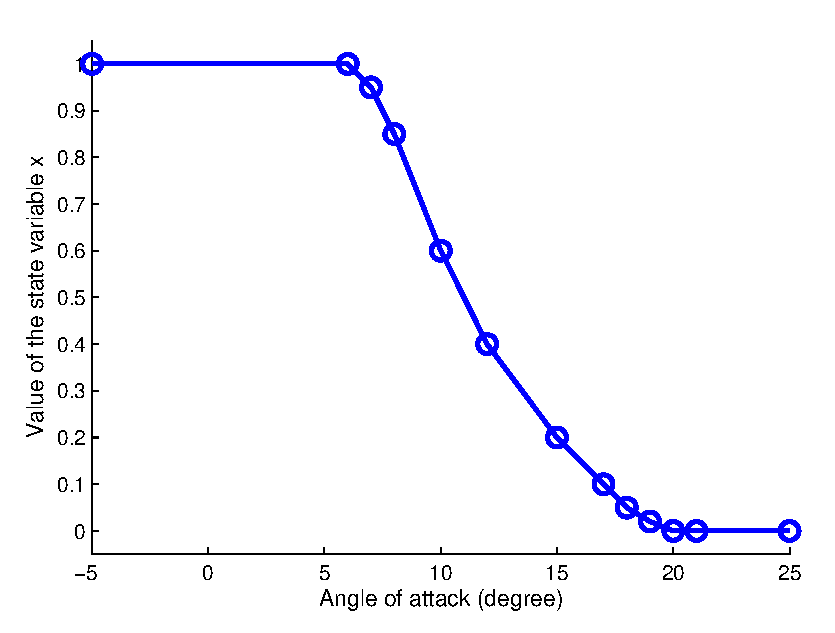
\includegraphics[width=1\textwidth]{./Figures/x_0_vs_alpha.eps}
      \end{center}
      \caption{Quasi-steady profile for the state variable $x$}
    \end{figure}
  \end{columns}
\end{frame}

\begin{frame}
  \frametitle{Time constant determination}
\end{frame}

\begin{frame}
  \frametitle{Comparison with periodic measurements}
\end{frame}

\begin{frame}
  \frametitle{Pseudo-random case}
\end{frame}


\section[Unsteady optimization]{Unsteady trajectory optimization}

\subsection{Time constant equivalence}

\begin{frame}
  \frametitle{Froude number equivalence}
\end{frame}

\subsection{Gust duration dependency}

\begin{frame}
  \frametitle{Global results}
\end{frame}

\begin{frame}
  \frametitle{Tg=0.5}
\end{frame}

\begin{frame}
  \frametitle{Tg=0.1}
\end{frame}


\subsection{Phase results}

\begin{frame}
  put Wa vs Tg curve and alpha tg to explain on the same slide?
\end{frame}

\section{Conclusion}

\end{document}
